\documentclass{book}
\usepackage{blindtext, hyperref, verbatim, minted, graphicx, amssymb, textcomp, enumerate, tcolorbox, newunicodechar, textgreek, wasysym, tipa, eso-pic, lipsum, bbold, dsfont}
\usepackage[margin=1.3in]{geometry}
\usepackage{longtable}
\usepackage{lmodern} % Add this line to use the Latin Modern font
\renewcommand\familydefault{\sfdefault}
\usepackage{fontspec}
\usepackage{newunicodechar}
\usepackage[utf8]{inputenc}
\usepackage{xcolor}

\usepackage{amsthm}

% Theorem styles
\newtheorem{theorem}{Theorem}[section]
\newtheorem{definition}[theorem]{Definition}

\newunicodechar{×}{$\times$}
\newunicodechar{→}{$\rightarrow$}
\newunicodechar{⟨}{$\langle$}
\newunicodechar{⟩}{$\rangle$}
\newunicodechar{↦}{$\mapsto$}
\newunicodechar{∧}{$\wedge$}
\newunicodechar{∨}{$\vee$}
\newunicodechar{∃}{$\exists$}
\newunicodechar{∀}{$\forall$}
\newunicodechar{¬}{$\neg$}

\newunicodechar{ᵃ}{${}^{\texttt{a}}$}
\newunicodechar{ᵇ}{${}^{\texttt{b}}$}
\newunicodechar{ᶜ}{${}^{\texttt{c}}$}
\newunicodechar{ᵈ}{${}^{\texttt{d}}$}
\newunicodechar{ᵉ}{${}^{\texttt{e}}$}
\newunicodechar{ᶠ}{${}^{\texttt{f}}$}
\newunicodechar{ᵍ}{${}^{\texttt{g}}$}
\newunicodechar{ʰ}{${}^{\texttt{h}}$}
\newunicodechar{ⁱ}{${}^{\texttt{i}}$}
\newunicodechar{ʲ}{${}^{\texttt{j}}$}
\newunicodechar{ᵏ}{${}^{\texttt{k}}$}
\newunicodechar{ˡ}{${}^{\texttt{l}}$}
\newunicodechar{ᵐ}{${}^{\texttt{m}}$}
\newunicodechar{ⁿ}{${}^{\texttt{n}}$}
\newunicodechar{ᵒ}{${}^{\texttt{o}}$}
\newunicodechar{ᵖ}{${}^{\texttt{p}}$}
\newunicodechar{ʳ}{${}^{\texttt{r}}$}
\newunicodechar{ˢ}{${}^{\texttt{s}}$}
\newunicodechar{ᵗ}{${}^{\texttt{t}}$}
\newunicodechar{ᵘ}{${}^{\texttt{u}}$}
\newunicodechar{ᵛ}{${}^{\texttt{v}}$}
\newunicodechar{ʷ}{${}^{\texttt{w}}$}
\newunicodechar{ˣ}{${}^{\texttt{x}}$}
\newunicodechar{ʸ}{${}^{\texttt{y}}$}
\newunicodechar{ᶻ}{${}^{\texttt{z}}$}

\newunicodechar{⁰}{${}^{\texttt{0}}$}
\newunicodechar{¹}{${}^{\texttt{1}}$}
\newunicodechar{²}{${}^{\texttt{2}}$}
\newunicodechar{³}{${}^{\texttt{3}}$}
\newunicodechar{⁴}{${}^{\texttt{4}}$}
\newunicodechar{⁵}{${}^{\texttt{5}}$}
\newunicodechar{⁶}{${}^{\texttt{6}}$}
\newunicodechar{⁷}{${}^{\texttt{7}}$}
\newunicodechar{⁸}{${}^{\texttt{8}}$}
\newunicodechar{⁹}{${}^{\texttt{9}}$}

\newunicodechar{⁻}{${}^{\texttt{-}}$}

\newunicodechar{ᵒ}{${}^{\texttt{o}}$}
\newunicodechar{ᵖ}{${}^{\texttt{p}}$}


\newunicodechar{ₑ}{${}_{\texttt{e}}$}


\newunicodechar{⁻}{${}^{\texttt{-}}$}
\newunicodechar{¹}{${}^{\texttt{1}}$}

\newunicodechar{₀}{${}_{\texttt{0}}$}
\newunicodechar{₁}{${}_{\texttt{1}}$}
\newunicodechar{₂}{${}_{\texttt{2}}$}
\newunicodechar{₃}{${}_{\texttt{3}}$}
\newunicodechar{₄}{${}_{\texttt{4}}$}
\newunicodechar{₅}{${}_{\texttt{5}}$}
\newunicodechar{₆}{${}_{\texttt{6}}$}
\newunicodechar{₇}{${}_{\texttt{7}}$}
\newunicodechar{₈}{${}_{\texttt{8}}$}
\newunicodechar{₉}{${}_{\texttt{9}}$}

\newunicodechar{𝚫}{$\Delta$}

\newunicodechar{𝔸}{$\mathbb{A}$}
\newunicodechar{𝔹}{$\mathbb{B}$}
\newunicodechar{ℂ}{$\mathbb{C}$}
%\newunicodechar{}{$\mathbb{D}$}
%\newunicodechar{}{$\mathbb{E}$}
%\newunicodechar{}{$\mathbb{F}$}
\newunicodechar{𝔾}{$\mathbb{G}$}
%\newunicodechar{}{$\mathbb{H}$}
%\newunicodechar{}{$\mathbb{I}$}
%\newunicodechar{}{$\mathbb{J}$}
%\newunicodechar{}{$\mathbb{K}$}
%\newunicodechar{}{$\mathbb{L}$}
%\newunicodechar{}{$\mathbb{M}$}
\newunicodechar{ℕ}{$\mathbb{N}$}
\newunicodechar{𝕆}{$\mathbb{O}$}
\newunicodechar{ℙ}{$\mathbb{P}$}
%\newunicodechar{}{$\mathbb{Q}$}
\newunicodechar{ℝ}{$\mathbb{R}$}
\newunicodechar{𝕊}{$\mathbb{S}$}
%\newunicodechar{}{$\mathbb{T}$}
%\newunicodechar{}{$\mathbb{U}$}
%\newunicodechar{}{$\mathbb{V}$}
%\newunicodechar{}{$\mathbb{W}$}
%\newunicodechar{}{$\mathbb{X}$}
%\newunicodechar{}{$\mathbb{Y}$}
\newunicodechar{ℤ}{$\mathbb{Z}$}
\newunicodechar{𝕒}{$\mathbb{a}$}
\newunicodechar{𝕓}{$\mathbb{b}$}
%\newunicodechar{}{$\mathbb{c}$}
\newunicodechar{𝕕}{$\mathbb{d}$}
\newunicodechar{𝕖}{$\mathbb{e}$}
%\newunicodechar{}{$\mathbb{f}$}
%\newunicodechar{}{$\mathbb{g}$}
%\newunicodechar{}{$\mathbb{h}$}
%\newunicodechar{}{$\mathbb{i}$}
\newunicodechar{𝕛}{$\mathbb{j}$}
%\newunicodechar{}{$\mathbb{k}$}
%\newunicodechar{}{$\mathbb{l}$}
%\newunicodechar{}{$\mathbb{m}$}
%\newunicodechar{}{$\mathbb{n}$}
\newunicodechar{𝕠}{$\mathbb{o}$}
\newunicodechar{𝕡}{$\mathbb{p}$}
%\newunicodechar{}{$\mathbb{q}$}
\newunicodechar{𝕣}{$\mathbb{r}$}
%\newunicodechar{}{$\mathbb{s}$}
\newunicodechar{𝕥}{$\mathbb{t}$}
%\newunicodechar{}{$\mathbb{u}$}
%\newunicodechar{}{$\mathbb{v}$}
%\newunicodechar{}{$\mathbb{w}$}
%\newunicodechar{}{$\mathbb{x}$}
%\newunicodechar{}{$\mathbb{y}$}
%\newunicodechar{}{$\mathbb{z}$}

\newunicodechar{⊣}{\ensuremath{\dashv}}
\newunicodechar{ॱ}{${}^{\cdot}$}
\newunicodechar{𛲔}{${}_{\cdot}$}
\newunicodechar{⇄}{$\rightleftarrows$}
\newunicodechar{⇆}{$\leftrightarrows$}



\newunicodechar{⌣}{$\cup$}


\newunicodechar{ꜝ}{$\raisebox{1ex}{\scalebox{0.5}{\texttt{!}}}$}
\newunicodechar{ꜞ}{$\raisebox{1ex}{\scalebox{0.5}{\texttt{¡}}}$}

\newunicodechar{𝟙}{$\mathbb{1}$}
\newunicodechar{∘}{$\circ$}

\newunicodechar{𝟏}{${\bold{1}}$}
\newunicodechar{⭢}{$\longrightarrow$}
\newunicodechar{•}{${\bullet}$}
\newunicodechar{∙}{${\bullet}$}

\newunicodechar{⇉}{$\rightrightarrows$}
\newunicodechar{よ}{$
\includegraphics[width=0.27cm,height=0.27cm]{yon.png}$}

\newunicodechar{∼}{$\sim$}
\newunicodechar{≃}{$\simeq$}
\newunicodechar{≅}{$\cong$}
\newunicodechar{∞}{$\infty$}


\newunicodechar{½}{$\frac{1}{2}$}


\newunicodechar{α}{$\alpha$}
\newunicodechar{β}{$\beta$}
\newunicodechar{γ}{$\gamma$}
\newunicodechar{δ}{$\delta$}
\newunicodechar{ε}{$\epsilon$}
\newunicodechar{η}{$\eta$}
\newunicodechar{ζ}{$\zeta$}
\newunicodechar{θ}{$\theta$}
\newunicodechar{ι}{$\iota$}
\newunicodechar{μ}{$\mu$}
\newunicodechar{κ}{$\kappa$}
\newunicodechar{λ}{$\lambda$}
\newunicodechar{ρ}{$\rho$}
\newunicodechar{π}{$\pi$}
\newunicodechar{σ}{$\sigma$}
\newunicodechar{τ}{$\tau$}
\newunicodechar{υ}{$\upsilon$}
\newunicodechar{φ}{$\phi$}
\newunicodechar{ψ}{$\psi$}
\newunicodechar{χ}{$\chi$}
\newunicodechar{ω}{$\omega$}

\makeatletter
\newcommand*{\shifttext}[2]{\settowidth{\@tempdima}{#2}\makebox[\@tempdima]{\hspace*{#1}#2}}
\makeatother
\definecolor{Red}{cmyk}{0.1, 0.70, 0.65, 0.00, 1.00}
\definecolor{Blue}{cmyk}{0.9, 0.2, 0.2, 0.00, 1.00}
\definecolor{Yellow}{cmyk}{0.0, 0.00, 0.7, 0.00, 0.5}
\definecolor{Green}{cmyk}{0.6, 0.0, 0.6, 0.00, 1.00}
\definecolor{Purple}{cmyk}{0.8, 0.3, 0.3, 0.00, 1.00}
\definecolor{Orange}{cmyk}{0.0, 0.3, 0.7, 0.00, 1.00}
\definecolor{Grey}{cmyk}{0.13, 0.13, 0.13, 0.00, 1.00}
\newcounter{definitioncounter}
\setcounter{definitioncounter}{1}
\newcounter{theoremcounter}
\setcounter{theoremcounter}{1}
\newcounter{printcounter}
\setcounter{printcounter}{1}
\newcounter{examplecounter}
\setcounter{examplecounter}{1}
\newcounter{ccounter}
\setcounter{ccounter}{1}
\newcounter{pcounter}
\setcounter{pcounter}{1}
\newcounter{lcounter}
\setcounter{lcounter}{1}
\newcounter{sectioncount}
\newcounter{subsectioncount}
\setcounter{sectioncount}{1}
\renewcommand{\section}[1]{\newpage\ \\ \ \\ \begin{center} \scalebox{1.5}{\texttt{\thesectioncount . #1}} \stepcounter{sectioncount} \setcounter{subsectioncount}{1} \end{center} \begin{center} \ \\ \ \\ \thispagestyle{empty} \end{center}}
\renewcommand{\subsection}[1]{\texttt{\thesubsectioncount . #1} \stepcounter{subsectioncount}}
\renewcommand{\backslash}{\reflectbox{\texttt{/}}}



\renewcommand{\section}[1]{
\newpage
{
\Huge 
\begin{center}
\ \\
\ \\
\thispagestyle{empty}
\texttt{#1}
\end{center}}
\ \\
\ \\
}
\begin{document}

\thispagestyle{empty} 

\AddToShipoutPicture*
    {\put(545,720){\href{http://www.linearlibrary.net}{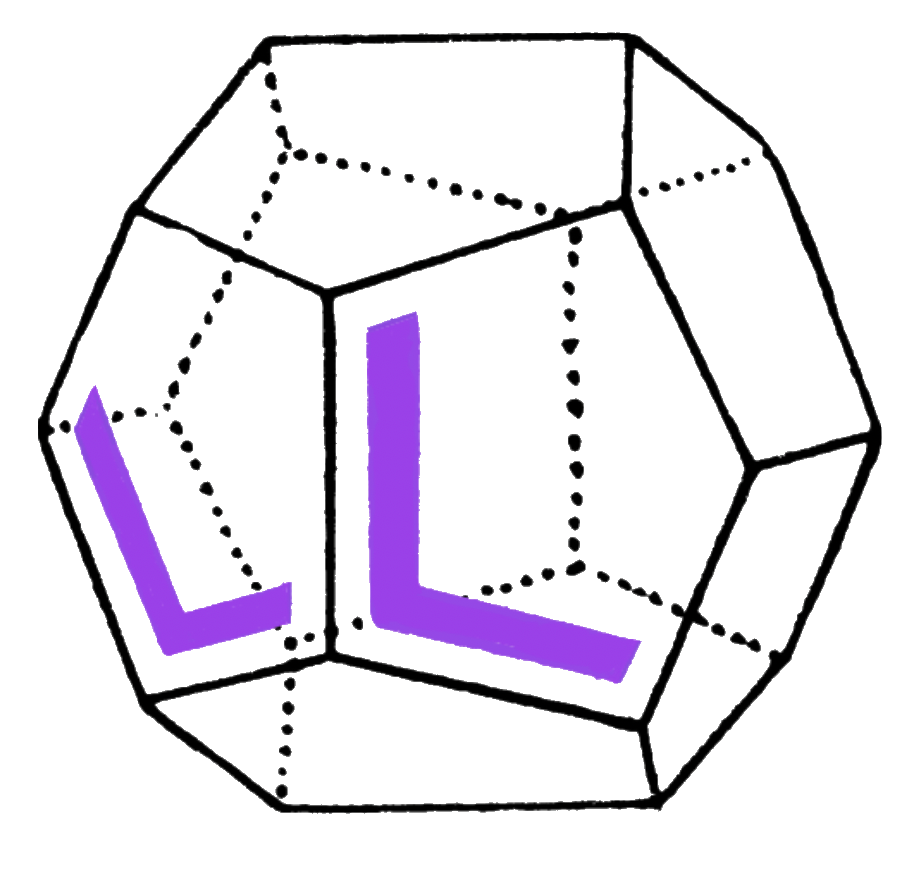
\includegraphics[width=2cm,height=2cm]{ll.png}}}}

\AddToShipoutPicture*
  {\put(465,767){\href{https://github.com/linlib/Chern-WeilTheory/blob/main/Chern-WeilTheory.py}{\raisebox{-0.198 em}{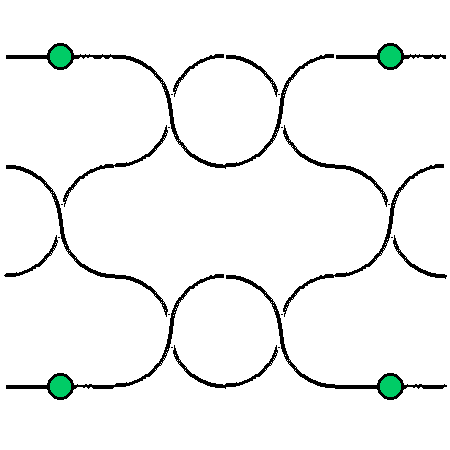
\includegraphics[width=0.35cm,height=0.35cm]{stringdiagrampicture.png}}\texttt{ Braid group}}}}

\AddToShipoutPicture*
  {\put(465,752){\href{https://ncatlab.org/nlab/show/HomePage}{\raisebox{-0.168 em}{
\includegraphics[width=0.33cm,height=0.33cm]{nlablogo.png}}\texttt{ nLab}}}}

\AddToShipoutPicture*
  {\put(465,737){\href{https://www.wikipedia.org}{\texttt{\raisebox{-0.158 em}{
\includegraphics[width=0.38cm,height=0.30cm]{wikipedialogo.png}} Wikipedia}}}}

  \AddToShipoutPicture*
  {\put(465,722){\href{https://github.com/CQTS}{\texttt{\raisebox{-0.178 em}{
\includegraphics[width=0.32cm,height=0.32cm]{cqtslogo.png}} CQTS}}}}


\AddToShipoutPicture*
  {\put(375,767){\href{https://github.com/linlib/Chern-WeilTheory/blob/main/Chern-WeilTheory.lean}{\texttt{\raisebox{-0.1 em}{
\includegraphics[width=0.30cm,height=0.30cm]{leanlogo.png}} Lean file}}}}

\AddToShipoutPicture*
  {\put(375,752){\href{https://github.com/linlib/Chern-WeilTheory/blob/main/Chern-WeilTheory.agda}{\texttt{\raisebox{-0.09 em}{
\includegraphics[width=0.33cm,height=0.31cm]{agdalogo.png}} Agda file}}}}

\AddToShipoutPicture*
  {\put(375,737){\href{https://github.com/linlib/Chern-WeilTheory/blob/main/Chern-WeilTheory.v}{\texttt{\raisebox{-0.17 em}{
\includegraphics[width=0.31cm,height=0.34cm]{coqlogo.png}} Coq file}}}}

  \AddToShipoutPicture*
  {\put(375,722){\href{https://github.com/linlib/Chern-WeilTheory/blob/main/Chern-WeilTheory.thy}{\texttt{\raisebox{-0.2 em}{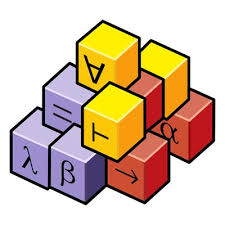
\includegraphics[width=0.34cm,height=0.35cm]{isabellelogo.png}} Isabelle file}}}}


\AddToShipoutPicture*
  {\put(281,767){\href{https://leanprover.zulipchat.com/}{\texttt{\raisebox{-0.1 em}{
\includegraphics[width=0.30cm,height=0.30cm]{leanlogo.png}} Lean Zulip}}}}

\AddToShipoutPicture*
  {\put(281,752){\href{https://agda.zulipchat.com}{\texttt{\raisebox{-0.09 em}{
\includegraphics[width=0.33cm,height=0.31cm]{agdalogo.png}} Agda Zulip}}\\
}}

\AddToShipoutPicture*
  {\put(281,737){\href{https://coq.zulipchat.com}{\texttt{\raisebox{-0.17 em}{
\includegraphics[width=0.31cm,height=0.34cm]{coqlogo.png}} Coq Zulip}}\\
}}

  \AddToShipoutPicture*
  {\put(281,722){\href{https://isabelle.zulipchat.com}{\texttt{\raisebox{-0.2 em}{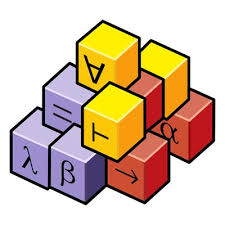
\includegraphics[width=0.34cm,height=0.35cm]{isabellelogo.png}} Isabelle Zulip}}}}


\AddToShipoutPicture*
  {\put(185,767){\href{https://linearlibrary.net}{\texttt{linearlibrary}}}}

\AddToShipoutPicture*
  {\put(185,752){\href{https://live.lean-lang.org}{\texttt{Leanprover}}}}

\AddToShipoutPicture*
  {\put(185,737){\href{https://github.com/linlib/Chern-WeilTheory/blob/main/Chern-WeilTheory.tex}{\texttt{Latex file}}}}

  \AddToShipoutPicture*
  {\put(185,722){\href{https://github.com/linlib/Chern-WeilTheory/blob/main/Chern-WeilTheory.pdf}{\texttt{PDF file}}
  }}

\ \\
\ \\
%LEAN: 
\begin{center}
\begin{tcolorbox}[width=2.64in,colback={white},coltitle=white]
\begin{center}
\scalebox{1.8}{\texttt{Chern-Weil Theory}}
\end{center}
\end{tcolorbox}
\end{center}

\iffalse
%LEAN: 
\begin{center}
\begin{tcolorbox}[width=5in,colback={white},colbacktitle=Blue,coltitle=black]
\begin{minted}[breaklines, escapeinside=||]{lean}

B²GL(ℂ) ≃ GL(ℂ)

\end{minted}
\end{tcolorbox}
\end{center}

\iffalse

\fi



\begin{center}
\href{https://live.lean-lang.org/#codez=CYUwZgBAzglgdgcwK4BsCGAnA+gYwPYAWeAtninggJ5Z5i4kAOKIAHlgiHCBmilivBCZ2GPEgZYA7jAAuBeuDAwcMTjKhZ4WDEL5wkxAEbcoEAFwQAKpQYhzAXgiHK0PBgyUAUJ7h4ZaGRg8OAgAIgAJQEdIAAoAcQAZQEyCaMAgQgBKABpAXEI00Ih7AD5oeGR0bHwiUnIqGjp8YiZWdk5uXn5BYQRRcSlZeXxFZVU4dU04bV0sfSMTb1BIHB6GUWAkHBlzCCi4pNTMnIhAJMItmITk9Oy0o5Od8/2rs0dnV3cvX39A4IgWMMBiYjyXIUIIsJMs8Kt1t8IF5PAA3TAwNCGZgQADeIKwYIhMk0oBGshcFm2Zz2lwAvnCEUiUeikBh4TI6SAsGA3MRNsTdhcchT4RhEci7KjAJPAHNOXPuFM8AHoALSeeYQHhwADWWAATOMdG0KiQyBRCVYbHZHk4XFA3B5vO8AkEQqFAJXAMQAwoBHAkA/gSAAtxogAhBKAY1w9plAKwbgBJd4OASl27rl8kVlWrNRMdYQ9dUYbLpXNwMCCJsAHIBa6cu6XTwAHwgAAYIDXazWgRisWscTA8YEZF4K9ECzIAHRQNY4CBwK5A6I4XMjiC/CDCoA}{chern class notation}

\end{center}

\ \\
\ \\
\thispagestyle{empty}

\iffalse
/-
def rank_2n_real_cohomology : Type := by sorry

notation "Ωॱ(Cⁱⁿᶠ(BGLᵣ(ℂ)),𝔤𝔩ₙ(ℂ))" => rank_2n_real_cohomology

-/
\fi

\ \\
\ \\
\ \\
\ \\
\ \\
\ \\
\ \\
\ \\
\ \\
\ \\
\ \\

\newpage
\pagecolor{white}
\color{black}
\ \\
\ \\
\thispagestyle{empty}
\large %%%%%%%% HERE IS THE large LARGE size textsize set text size
\newpage 
\ \\
\ \\
\ \\
\ \\
\ \\
\ \\
\ \\
\ \\
\ \\
\ \\
\ \\
\thispagestyle{empty}
\fi


\newpage
\section{Contents}

{
\footnotesize
\begin{longtable}{|| l || l ||} 
\hline
\multicolumn{1}{|c|}{$\texttt{Section}$} & \multicolumn{1}{|c|}{$\texttt{Description}$} \\
\hline
Introduction &  \\
\hline
Contents &  \\
\hline
Unicode &  \\
\hline \hline
\multicolumn{2}{||c||}{\texttt{BIBLIOGRAPHY}} \\
\hline \hline
 & \\
\hline \hline
\end{longtable}
}


\newpage
\subsection{Notes}

% https://ncatlab.org/nlab/show/Introduction+to+Cobordism+and+Complex+Oriented+Cohomology


{
\footnotesize
\begin{longtable}{|| l || l ||} 
\hline 
\multicolumn{1}{|c|}{$\texttt{...}$} & \multicolumn{1}{|c|}{$\texttt{EXAMPLE2}$} \\
\hline \hline
 &  \\
\hline
 &  \\
\hline
 &  \\
\hline 
\end{longtable}
}


\newpage
\subsection{Unicode}

Lean 4 uses unicode, and this entails an extensive catalogue of characters to choose from. Here is a list of the unicode characters we will use:

{\footnotesize
\begin{center}
\begin{tabular}{|| l || l || l || l ||} 
\hline
$\texttt{Symbol}$ & $\texttt{Unicode}$ & \texttt{VSCode shortcut} & $\texttt{Use}$\\
\hline
\hline
\multicolumn{4}{||c||}{\texttt{Lean's Kernel}} \\
\hline
\hline
× & 2A2F & \backslash\texttt{times} & Product of types\\
\hline
→ & 2192 & \backslash\texttt{rightarrow}  & Hom of types\\
\hline
⟨,⟩ & 27E8,27E9 & \backslash\texttt{langle},\backslash\texttt{rangle}  & Product term introduction\\
\hline
↦ & 21A6 &\backslash\texttt{mapsto}  & Hom term introduction\\
\hline
∧ & 2227 &\backslash\texttt{wedge}  & Conjunction \\
\hline
∨ & 2228 &\backslash\texttt{vee}  & Disjunction \\
\hline
∀ & 2200 &\backslash\texttt{forall}  & Universal quantification \\
\hline
∃ & 2203 &\backslash\texttt{exists}  & Existential quantification\\
\hline
¬ & 00AC &\backslash\texttt{neg}  & Negation\\
\hline
\hline
\multicolumn{4}{||c||}{\texttt{Variables and Constants}} \\
\hline
\hline
\iffalseᵃ,ᵇ,ᶜ,...,ᶻ \fi & 1D52,1D56 & \iffalse \backslash\wedge\texttt{a},\backslash\wedge\texttt{b},\backslash\wedge\texttt{c},...\backslash\wedge\texttt{z} \fi  & Variables and constants \\
\hline
\iffalse ⁰,¹,²,³,⁴,⁵,⁶,⁷,⁸,⁹ \fi & 1D52,1D56 & \iffalse \backslash\wedge\texttt{0},\backslash\wedge\texttt{1},\backslash\wedge\texttt{2},...,\backslash\wedge\texttt{9} \fi  & Variables and constants \\
\hline
⁻ & 207B & \iffalse \backslash\wedge\texttt{-},  \fi & Variables and constants \\
\hline
₀,₁,₂,₃,₄,₅,₆,₇,₈,₉ & 2080 - 2089 &\backslash\texttt{0}-\backslash\texttt{9} & Variables and constants\\
\hline
\texttt{α}-\texttt{ω},\texttt{A}-\texttt{Ω} & 03B1-03C9 & & Variables and constants\\
\hline
\hline
 \multicolumn{4}{||c||}{\texttt{Adjunctions}} \\
\hline
\hline
⇄ & 21C4 & \backslash\texttt{rightleftarrows}  & Adjunctions \\
\hline
⇆ & 21C6 & \backslash\texttt{leftrightarrows}  & Adjunctions \\
\hline
𛲔 & 1BC94 &  & Right adjoints\\
\hline
ॱ & 0971 &  & Left adjoints \\
\hline
⊣ & 22A3 & \backslash\texttt{dashv}  & The condition that two Functors are adjoint \\
\hline
\multicolumn{4}{||c||}{\texttt{Miscellaneous}} \\
\hline
\hline
∼ & 223C & \backslash\texttt{sim} & Homotopies \\
\hline
≃ & 2243 & \backslash\texttt{equiv}  & Equivalences \\
\hline
≅ & 2245 & \backslash\texttt{cong}  & Isomorphisms \\
\hline
∞ & 221E & \backslash\texttt{infty}  & Infinity categories and infinity groupoids\\ 
\hline
 \hline
\end{tabular}
\end{center}}




\newpage
\begin{center}
\texttt{BIBLIOGRAPHY}
\end{center}
\newpage
\thispagestyle{empty}

\begin{enumerate}
\item 
\end{enumerate}


\end{document}


